Another way to analyze log data is to view the log as a sequence of events occurring in a state machine.  Using state models, we can quantify the occurrences of repeating actoins and describe a usage pattern in statistical analysis.  In state model analysis, the sequential data is converted to nodes and edges of a graph which represents the entire data in states and transitions between them.  A Markov state model provides information about the probability of occurrence of each state and the transitional probability of each activity.   The statisics provided in a Markov state model include the quantity of time and probability for the developer being in each state.  From a given state, the model calculates the probability of each transition to different unique states.  State models answer specific questions such as what is the probability that once a developer searches the code, they edit a code element listed in the find results. Expanding this question, the probability of an entire use case or set of transitions through the usage model, is caclulable from the state model.  

State model graphs make it easy to identify the most active states and edges provides information about the important activities in the data set.  As the number of states increases, the WDG becomes more complex and hence difficult to understand.  When this occurrs, summarizing the detailed event data into higher-level categories effectively combines the states to get more meaningful information.   For example, classifing events in usage data of similar types into categories results in fewer states with the same number of transitions as the orignial data.

We generate a state model from a usage log by transforming the serially ordered events in a sequence data to a Weighted Directed Graph (WDG) data structure.  We can abstract the information in the log line to any level, such as, event level, event category level, tool level, or application level. In the sequence data, each event is important as a standalone event, however, in the WDG representation, the importance shifts to adjacent pairs of events. 
%We do this type of a transformation to record the order in which events happened. 
Therefore, each unique event in the sequence data is represented by a unique node in the WDG. 

To understand how to interpret a state model, look at our example graph figure \ref{op-profile-example}.  We see that an edge exists from one node (head) to another (tail) if there is an occurrence of the event representing the tail node immediately after the event representing the head node in the  log file. For example if event B follows event A in the log file, then there is directed edge from node A to node B in the WDG. The edges are labeled with the number of times this transition has occurred.  For example if B occurs a fifty times after A in the log file, then the edge from node A to node B in the WDG is labeled with 50. Typically, we keep track of the actual count as the weight of the edge, when building the graph. In the graph we display the percentage value as the label. This percentage is proportional to the total number of transitions.  The cumulative probability of out-edges of a node is 1. The transitional probabilities of each out-edge is calculated by dividing the number of transactions of that out-edge with the sum of all outward transactions from that node. We could also store the dynamic parameter information in each log line as a list along the edges. 

As an example, consider a sample log file shown in figure \ref{samplelogfile} given below and the corresponding state model graph in figure \ref{op-profile-example}. Intuitively you can see how the state model represents the log states and transitions between them in the sequence of events.  

\begin{figure}
\hrulefill
\begin{verbatim}
2013-03-21 18:18:32Z,A
2013-03-21 18:18:33Z,B
2013-03-21 18:20:49Z,C
2013-03-21 18:20:50Z,A
2013-03-21 18:20:56Z,B
2013-03-21 18:20:57Z,A
2013-03-21 18:21:08Z,C
2013-03-21 18:21:08Z,D
2013-03-21 18:21:08Z,E
2013-03-21 18:21:08Z,A
\end{verbatim}
\hrulefill
\caption{Sample Log File to Convert to State Model}\label{samplelogfile}
\end{figure}

\begin{figure}[h]
  \centering
  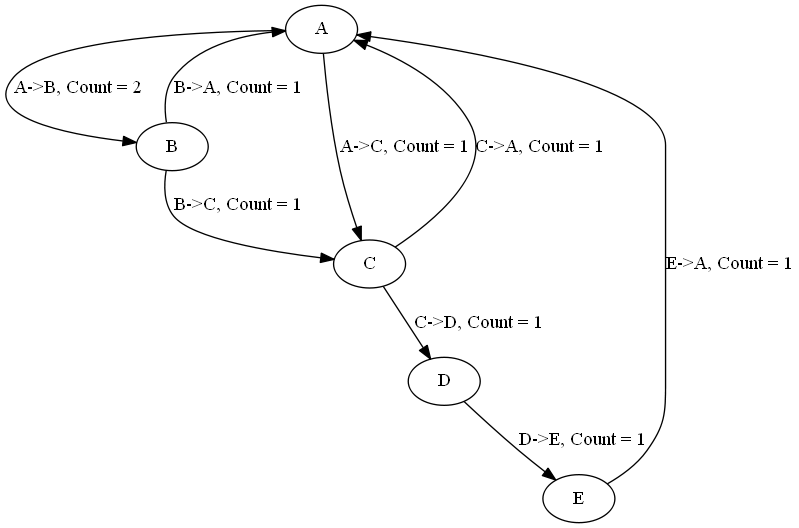
\includegraphics[scale=.40]{op-profile-example.png}
  \caption{Weighted Directed Graph of the Example Log}\label{op-profile-example}
\end{figure}






%the other example is aligned with the sample graph thus better.
%As an example of WDG, consider a simple log file where the activities are separated by commas. $1-2, 2-3, 3-4, 4-5, 5-4, 4-5, 5-4, 4-6, 6-7, 7-5, 5-4, 4-5, 5-4, 4-5, 5-8, 8-9$. The events in the log file are mapped to their corresponding event IDs: $1, 2, 3, 4, 5, 4, 5, 4, 6, 7, 5, 4, 5, 4, 5, 8, 9$. Each node is a unique event. An edge between nodes 1 and 2 signifies that the event 2  appears after event 1  in the log file. The labels on the edges have the actual count and could have the transitional probabilities as well. The transitional probability from node 1 to node 2 is 1.0, whereas the transitional probability from node 4 to node 6 is 0.2.  This is depicted in Fig \ref{op-profile-example}.
 
Converting a log into a state model requires three steps.  We use JUMBL (Java Usage Model Builder) from the Software Quality Reasearch Laboratory (SQRL) of the University of Tennessee.    Details on input formats and JUMBL tools are available on sourceforge at \footnote{\url{http://jumbl.sourceforge.net/}}.
\begin{enumerate}
\item
First, convert the log file into a representation for each transition called a sequence based specification. The format for a sequence based specficicaiton in csv files is described in the JUMBL user guide. This representation contains the following information with one row for each transition :
\begin{itemize}
\item State transition
\item Count of transitions
\item Total time elapsed
\item State In information
\item State Out information
\end{itemize}

\item
After importing the sequence based spec, JUMBL can write out the representation of a state model as a TML script or several other formats including GML (Graph Modeling Language) that graph tools can import.  The TML  has information about the nodes, the out edges from each node along with the number of transitions from each node to another. The corresponding graph for the usage log example is depicted in Fig. \ref{op-profile-example}
\end{enumerate}


Using state models, a sequence data with hundreds of thousands of lines can be quickly converted to more meaningful graphical representation using this method. Once the TML file is generated, we can use JUMBL to find out the state probabilities of each states. Using the state probability and the usage patterns we can draw conclusions about the occupancy of individual states and the use cases that involve transitions through several states.

%Trying this on without the following examples.  They don't really add much and raise more questions than they answer.  I hope reference take care of the how to in this case.


%
%\begin{figure}
%\label{sampleTML}
%\hrulefill
%\begin{verbatim}
%($ fill(1) $)
%model testlog
%//use this before each transition to show probability ($0.10$)
%
%source [A]
%($2$)"Count=2 (A->B), TimeElapsed= 7secs" [B]
%($1$)"Count=1 (A->C), TimeElapsed= 11secs" [C]
%
%[B]
%($1$)"Count=1 (B->C), TimeElapsed= 136secs" [C]
%($1$)"Count=1 (B->A), TimeElapsed= 1secs" [A]
%
%[C]
%($1$)"Count=1 (C->A), TimeElapsed= 1secs" [A]
%($1$)"Count=1 (C->D)" [D]
%
%[D]
%($1$)"Count=1 (D->E)" [E]
%
%[E]
%($1$)"Count=1 (E->A)" [A]
%
%
%"exit" [Exit]
%
%end 
%\end{verbatim}
%\hrulefill
%\caption{Sample TML for a State Model}
%\end{figure}



%%I commented these out because they were out in space in the document and not well supported by the text.  You probably cut the text because of other comments.  Anyhow does it make sense to stick with one WDG example based on the state model shown in text above?  Seems OK to me so far. 

%\begin{figure}
%  \centering
%  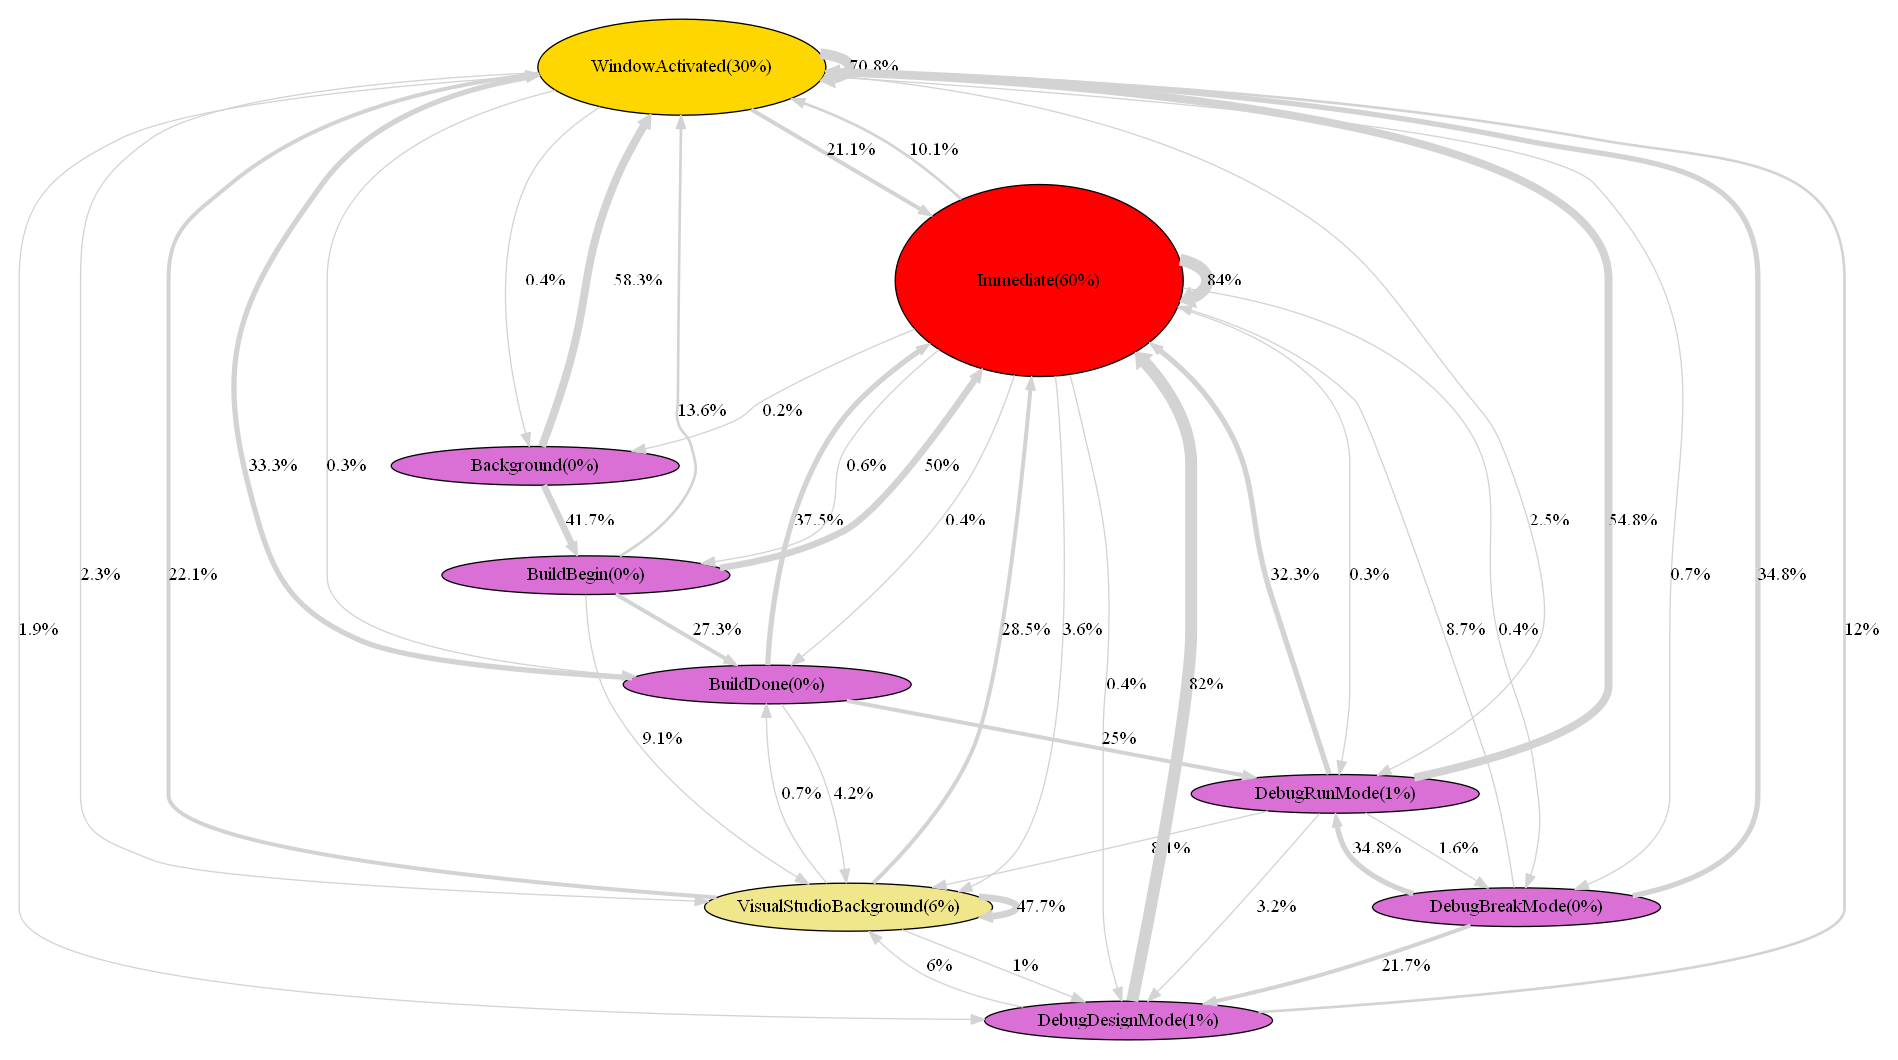
\includegraphics[scale=.15]{log_with_color.png}
%  \caption{WDG example with probability}\label{fig:log_with_color}
%\end{figure}

%\begin{figure}
%  \centering
%  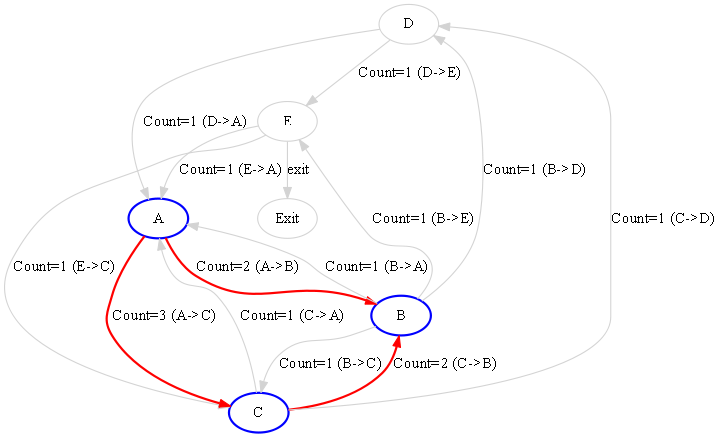
\includegraphics[scale=.50]{sample_log.png}
%  \caption{WDG example with count}\label{fig:sample_log}
%\end{figure}

 


